\subsection{Differenzieren Trigonometrischer Funktionen}

\begin{figure}[H]
    \centering
    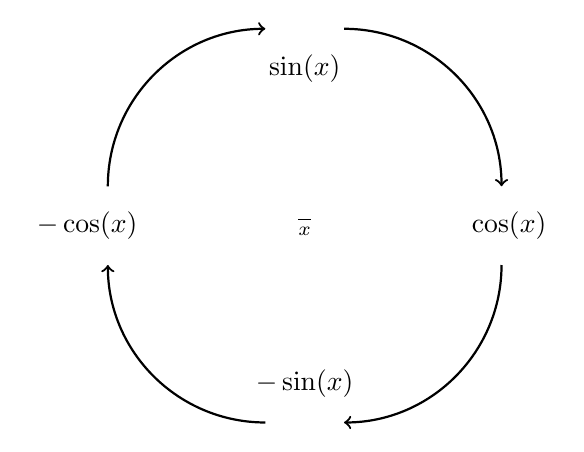
\begin{tikzpicture}
        \node at (0,0) {\( \sin(x) \)};
        \node[right] at (2,-2) {\( \cos(x) \)};
        \node at (0,-4) {\( -\sin(x) \)};
        \node[left] at (-2,-2) {\( -\cos(x) \)};

        \draw[->, thick] (0.5,0.5) arc (-270: -360: 2);
        \draw[->, thick] (2.5,-2.5) arc (0: -90: 2);
        \draw[->, thick] (-0.5,-4.5) arc (-90: -180: 2);
        \draw[->, thick] (-2.5,-1.5) arc (-180: -270: 2);

        \node[] at (0,-2) {\( \frac{\diff}{\diff x} \)};
    \end{tikzpicture}
    \caption{Der Ableitungskreis für Sinus \& Cosinus}
\end{figure}

\subsubsection{Sinus}

\begin{align*}
    & \limtozero{\Delta x} \frac{\sin(x_0 + \Delta x) - \sin(x_0)}{\Delta x} \\
    &= \limtozero{\Delta x} \frac{\sin(x_0) \cdot \cos(\Delta x) + \cos(x_0) \cdot \sin(\Delta x) - \sin(x_0)}{\Delta x} \\
    &= \limtozero{\Delta x} \underbrace{\sin(x_0)}_{\text{A}} \underbrace{\frac{\cos(\Delta x) - 1}{\Delta x}}_{\text{B}} +
    \limtozero{\Delta x} \underbrace{\cos(x_0)}_{\text{A}} \underbrace{\frac{\sin(\Delta x)}{\Delta x}}_{\text{B}} \\
    \\
    \text{A:\;} & \text{fester Wert} \\
    \text{B:\;} & \text{unbestimmter Ausdruck} \\
    \\
    &= \sin(x_0) \limtozero{\Delta x} \frac{\cos(\Delta x) - 1}{\Delta x} + \cos(x_0) \limtozero{\Delta x} \frac{\sin(\Delta x)}{\Delta x} \\
    &= \sin(x_0) \limtozero{\Delta x} \frac{(\cos(\Delta x) - 1) \cdot (\cos(\Delta x) + 1)}{\Delta x \cdot (\cos(\Delta x) + 1)} + \cdots \\
    &= \sin(x_0) \limtozero{\Delta x} \frac{\cos^2(\Delta x) - 1}{\Delta x \cdot (\cos(\Delta x) + 1)} + \cdots \\
    &= \sin(x_0) \limtozero{\Delta x} \frac{- \sin^2(\Delta x) - 1}{\Delta x \cdot (\cos(\Delta x) + 1)} + \cdots \\
    &= -\sin(x_0) \limtozero{\Delta x} \sin(\Delta x) \cdot \limtozero{\Delta x} \frac{\sin(\Delta x)}{\Delta x (\cos(\Delta x) + 1)} + \cdots \\
    &= \text{usw.}
\end{align*}

\subsubsection{Cosinus}

\begin{align*}
    y &= \cos(x) \\
    &= \sin(x + \frac{\pi}{2}) = \sin(z), &&\mid z = x + \frac{\pi}{2} \\
    & &&\mid \frac{\diff y}{\diff z} = \cos(z),\ \frac{\diff z}{\diff x} = 1 \\
    y' &= \cos\left(x + \frac{\pi}{2}\right) = -\sin(x) 
\end{align*}

\subsubsection{Tangens}

\begin{align*}
    y &= \tan(x) = \frac{\sin(x)}{\cos(x)} \\
    y' &= \frac{\cos(x)\cos(x) - \sin(x)\cdot (-\sin(x))}{\cos^2(x)} \\
    &= \frac{\cos^2(x) + \sin^2(x)}{\cos^2(x)} \\
    &= \frac{1}{\cos^2(x)} = 1 + \tan^2(x)
\end{align*}

\subsubsection{Cotangens}

\begin{align*}
    y &= \cot(x) = {(\tan(x))}^{-1} &&\mid z = \tan(x) \\
    & &&\mid \frac{\diff z}{\diff x} = \frac{1}{\cos^2(x)},\ \frac{\diff y}{\diff z} = -z^{-2} \\
    y' &= \frac{1}{\cos^2(x)} \cdot \left( -\frac{1}{\tan^2(x)} \right) \\
    &= -\frac{1}{\cos^2(x) \frac{\sin^2(x)}{\cos^2(x)}} \\
    &= -\frac{1}{\sin^2(x)} = -\left( 1 + \cot^2(x) \right)
\end{align*}

\subsubsection{Arkussinus}

\begin{align*}
    y &= \arcsin(x) &&\mid \sin() \\
    \sin(y) &= \sin(\arcsin(x)) = x &&\mid \frac{\diff x}{\diff y} = \cos(y) \Rightarrow \frac{\diff y}{\diff x} = \frac{1}{\cos(y)} = \frac{1}{\sqrt{1 - \sin^2(y)}} \\
    y' &= \frac{1}{\sqrt{1 - x^2}}
\end{align*}

\subsubsection{Arkuscosinus}

\begin{align*}
    y &= \arccos(x) &&\mid \cos() \\
    \cos(y) &= x &&\mid \frac{\diff x}{\diff y} = -\sin(y) \Rightarrow \frac{\diff y}{\diff x} = \frac{1}{-\sin(y)} = \frac{1}{\sqrt{1 - \cos^2(y)}} \\
    y' &= -\frac{1}{\sqrt{1 - x^2}} 
\end{align*}

\subsubsection{Arkustangens}

\begin{align*}
    y &= \arctan(x) &&\mid \tan() \\
    \tan(y) &= x &&\mid \frac{\diff x}{\diff y} = 1 + \tan^2(y) \Rightarrow \frac{\diff y}{\diff x} = \frac{1}{1 + \tan^2(y)} \\
    y' &= \frac{1}{1 + x^2}
\end{align*}

\subsubsection{Arkuskotangens}

\begin{align*}
    y &= \arccot(x) &&\mid \cot() \\
    \cot(y) &= x &&\mid \frac{\diff x}{\diff y} = 1 + \cot^2(y) \Rightarrow \frac{\diff y}{\diff x} = -\frac{1}{1 + \cot^2(y)} \\
    y' &= -\frac{1}{1 + x^2}
\end{align*}

